\documentclass[11pt,a4paper]{article}
\usepackage{amsmath,amssymb,amsfonts}
\usepackage[margin=1in]{geometry}
\usepackage{booktabs}
\usepackage{graphicx}
\usepackage[font=small,labelfont=bf]{caption}
\usepackage{microtype}
\usepackage{xcolor}
\usepackage[colorlinks=true,linkcolor=black,citecolor=black,urlcolor=blue]{hyperref}

\def\R{\mathbb{R}}
\def\E{\mathbb{E}}
\def\N{\mathcal{N}}
\def\xib{\boldsymbol{\xi}}

\title{Experiments: a rebuilt evaluation of Gaussian random-bridges\\
\large Working draft --- internal, verbose by design}
\author{}
\date{\today}

\begin{document}
\maketitle

\begin{abstract}
\noindent
This document records a complete re-implementation and re-measurement of the
empirical section. Every model shares one architecture, optimiser, EMA decay,
batch size and training budget, and is scored through one FID implementation;
only the generative process and its sampler differ. Three conclusions change
relative to the submitted manuscript. First, the reported step-count plateau is
an artefact of the sampler that was evaluated, not a property of the method:
with a correct sampler, quality improves monotonically to 1000 network
evaluations. Second, at matched budget the bridge now \emph{beats} improved
denoising diffusion at every step count, reversing the concession in the current
draft. Third, the free parameter is $\gamma^2=\sigma^2T$, not $\sigma$ and $T$
separately, which collapses two reported tuning decisions into one. We also
record several defects we found in our own re-implementation, because two of
them flattered the proposed method and would have survived review.
\end{abstract}

\section{Protocol}

\paragraph{What is held fixed.} One UNet per dataset, with parameter count
verified identical to the architecture used in the original experiments
(7.28\,M on MNIST, 52.54\,M on CIFAR-10). AdamW at $2\times10^{-4}$, 500-step
linear warmup then constant, gradient-norm clipping at 1.0, batch size 128,
40\,000 steps, EMA of the weights at decay 0.9999 with a ramp-in, bfloat16
autocast. All data at $32\times32$ in $[-1,1]$. Sampling and evaluation code is
shared by every method.

\paragraph{What FID means here.} 50\,000 generated samples per entry on MNIST,
scored against Inception-v3 pool3 statistics computed over the \emph{full}
60\,000-image training split. Generated samples are mapped once from $[-1,1]$ to
8-bit by a clamped affine map; no per-image rescaling is applied to either reals
or fakes, and nothing is written to disk in between.

This differs from the original pipeline in ways that matter. There, each sample
was min--max rescaled, written to PNG through \texttt{matplotlib} (which
normalises a second time, per image), read back, and min--max rescaled a third
time; reals received a per-image min--max as well. Per-image contrast
normalisation is not measurement-neutral, and the composite is not FID as it is
reported elsewhere. As an aside we note that the pipeline is \emph{contrast
blind}: the same image presented at four times the contrast maps to a
byte-identical array.

\paragraph{What the numbers can resolve.} FID is biased upward at finite sample
count, so we measure the floor rather than assume it. Comparing two disjoint
\emph{real} subsets of the same size gives, on MNIST, 6.89 at $n=2000$, 2.74 at
$n=5000$, 1.43 at $n=10\,000$ and 0.63 at $n=25\,000$. The figure quoted with the
main table, 0.15, is the matched floor: a real held-out set of 5000 against the
statistics of the remaining 55\,000, which is the structure of the model
measurement. Repeated sampling seeds give a standard deviation of 0.01--0.07 on
the headline entries, so differences above roughly $0.2$ are real and anything
smaller is not.

\section{Does quality improve with sampling steps?}

This is the question the submitted manuscript leaves open, describing a
``numerical plateauing behaviour'' to be investigated in future. It does not
require future work; it is the sampler.

\paragraph{The sampler that was evaluated.} \texttt{sample\_bridges.py}
constructs the sampler with \texttt{deterministic=True}, which deletes the
diffusion term from
\begin{equation}
\mathrm{d}\xib_s=\frac{\E[Y\mid\xib_s]-\xib_s}{1-s}\,\mathrm{d}s+\gamma\,\mathrm{d}B_s ,
\end{equation}
leaving $\xib_u=\xib_s+\frac{\hat y-\xib_s}{1-s}(u-s)$. Algorithm 2 of the
manuscript includes the diffusion term, so the published table was not produced
by the algorithm the paper prints. More importantly, the deletion is not a
harmless approximation. A deterministic sampler preserving the marginals must
follow the probability-flow ODE, whose drift carries the extra term
$-\tfrac{\gamma^2}{2}\nabla\!\log p_s$; without it the scheme matches neither
the SDE nor its flow ODE, and refining the grid converges to the wrong law.

\paragraph{Isolated, with no network involved.} On a one-dimensional problem
where $\E[Y\mid\xi_s]$ is available in closed form ($\Phi=\N(0,1)$, $\Psi$ a
Gaussian mixture), so that all residual error is the sampler's, the exact
posterior and Euler--Maruyama schemes both reach the Monte-Carlo floor in
1-Wasserstein distance at 2000 steps (0.0096 and 0.0095 against a floor of
0.0091), while the deterministic map stalls at 0.0625 --- $6.9\times$ the floor
--- with a persistent terminal variance deficit (1.726 against 1.758). The
residual scales with $\gamma$ exactly as the omitted score term predicts:
$1.2\times$ the floor at $\gamma=0.032$, $6.9\times$ at $0.316$, $41.9\times$ at
$1.0$, and $114\times$ at $\gamma=2$, where the terminal standard deviation
collapses from 1.758 to 0.775.

\paragraph{On images.} Table~\ref{tab:main} and Figure~\ref{fig:curves} carry
the same signature. The correct samplers fall monotonically to 1000 network
evaluations; the deterministic map converges to roughly three times their floor
excess and stays there.

\paragraph{What this does not explain.} The submitted table does not merely
plateau, it \emph{degrades}: 19.34 at 10 steps, 22.01 at 100, 23.55 at 1000.
Our deterministic sampler flattens but never worsens, so the sampler alone does
not account for the published curve. We tested two further hypotheses and both
failed. Degenerate time conditioning (Section~\ref{sec:defects}) shifts the
asymptote by $+0.4$ to $+0.6$ FID but produces a rise past the optimum of only
$+0.06$ to $+0.18$, against seed noise of $0.08$, where the published curve
climbs $+4.21$. Terminal-point precision is not implicated either: re-running
the original $t\in[0,T]$ grid in float64, and in the $s=t/T$ parameterisation,
changes the result by about one per cent at every step count. We therefore
report the \emph{level} and the \emph{plateau} as explained and attributed, and
the degradation as unexplained.

\section{Results at matched budget}

\begin{table}[t]
\centering\small
\caption{FID on MNIST against sampling steps, which equal network evaluations.
Shared architecture, optimiser, EMA, batch size and budget; identical evaluation
code. 50\,000 samples per entry, floor 0.15. Mean $\pm$ sd over sampling seeds
where repeats were run. \emph{This table is generated directly from the
evaluation output, not transcribed.}}
\label{tab:main}
\begin{tabular}{lccccccccc}
\toprule
Model & \multicolumn{9}{c}{Sampling steps (NFE)} \\
\cmidrule(lr){2-10}
 & 1 & 2 & 5 & 10 & 20 & 50 & 100 & 200 & 1000 \\
\midrule
Bridge (exact posterior) & 346.04 & 50.31 & \textbf{9.62} & 4.08 $\pm$ 0.06 & 2.14 & 1.37 $\pm$ 0.00 & 1.19 & 1.12 $\pm$ 0.00 & -- \\
Bridge (Euler-Maruyama) & \textbf{239.79} & 80.66 & 12.85 & \textbf{3.39 $\pm$ 0.03} & \textbf{1.74} & 1.26 $\pm$ 0.02 & 1.15 & 1.13 $\pm$ 0.02 & 1.06 \\
Bridge (deterministic Euler) & 246.18 & \textbf{45.28} & 10.32 & 5.78 $\pm$ 0.06 & 4.30 & 3.42 $\pm$ 0.05 & 3.19 & 2.95 $\pm$ 0.04 & -- \\
Flow matching & 298.68 & 54.09 & 10.34 & 4.13 $\pm$ 0.06 & 2.05 & \textbf{1.23 $\pm$ 0.02} & \textbf{1.07} & \textbf{1.02 $\pm$ 0.01} & \textbf{1.02} \\
DDPM cosine + DDIM & 418.50 & 380.07 & 17.76 & 6.96 & 4.07 & 2.24 & 1.40 & 2.83 & 16.30 \\
DDPM cosine ancestral & 377.15 & 380.14 & 16.27 & 9.01 & 4.83 & 3.00 & 2.90 & 2.99 & 2.71 \\
DDPM linear + DDIM & 418.36 & 285.10 & 14.05 & 7.22 & 4.48 & 2.79 & 1.67 & 2.74 & 13.26 \\
DDPM linear ancestral & 282.19 & 284.25 & 18.14 & 10.85 & 6.87 & 3.94 & 3.19 & 3.07 & -- \\
Improved DDPM (ancestral) & 389.46 & 393.23 & 20.06 & 10.99 & 7.16 & 3.62 & 2.02 & 1.74 & 1.93 \\
\bottomrule
\end{tabular}

\end{table}

\begin{figure}[t]
\centering
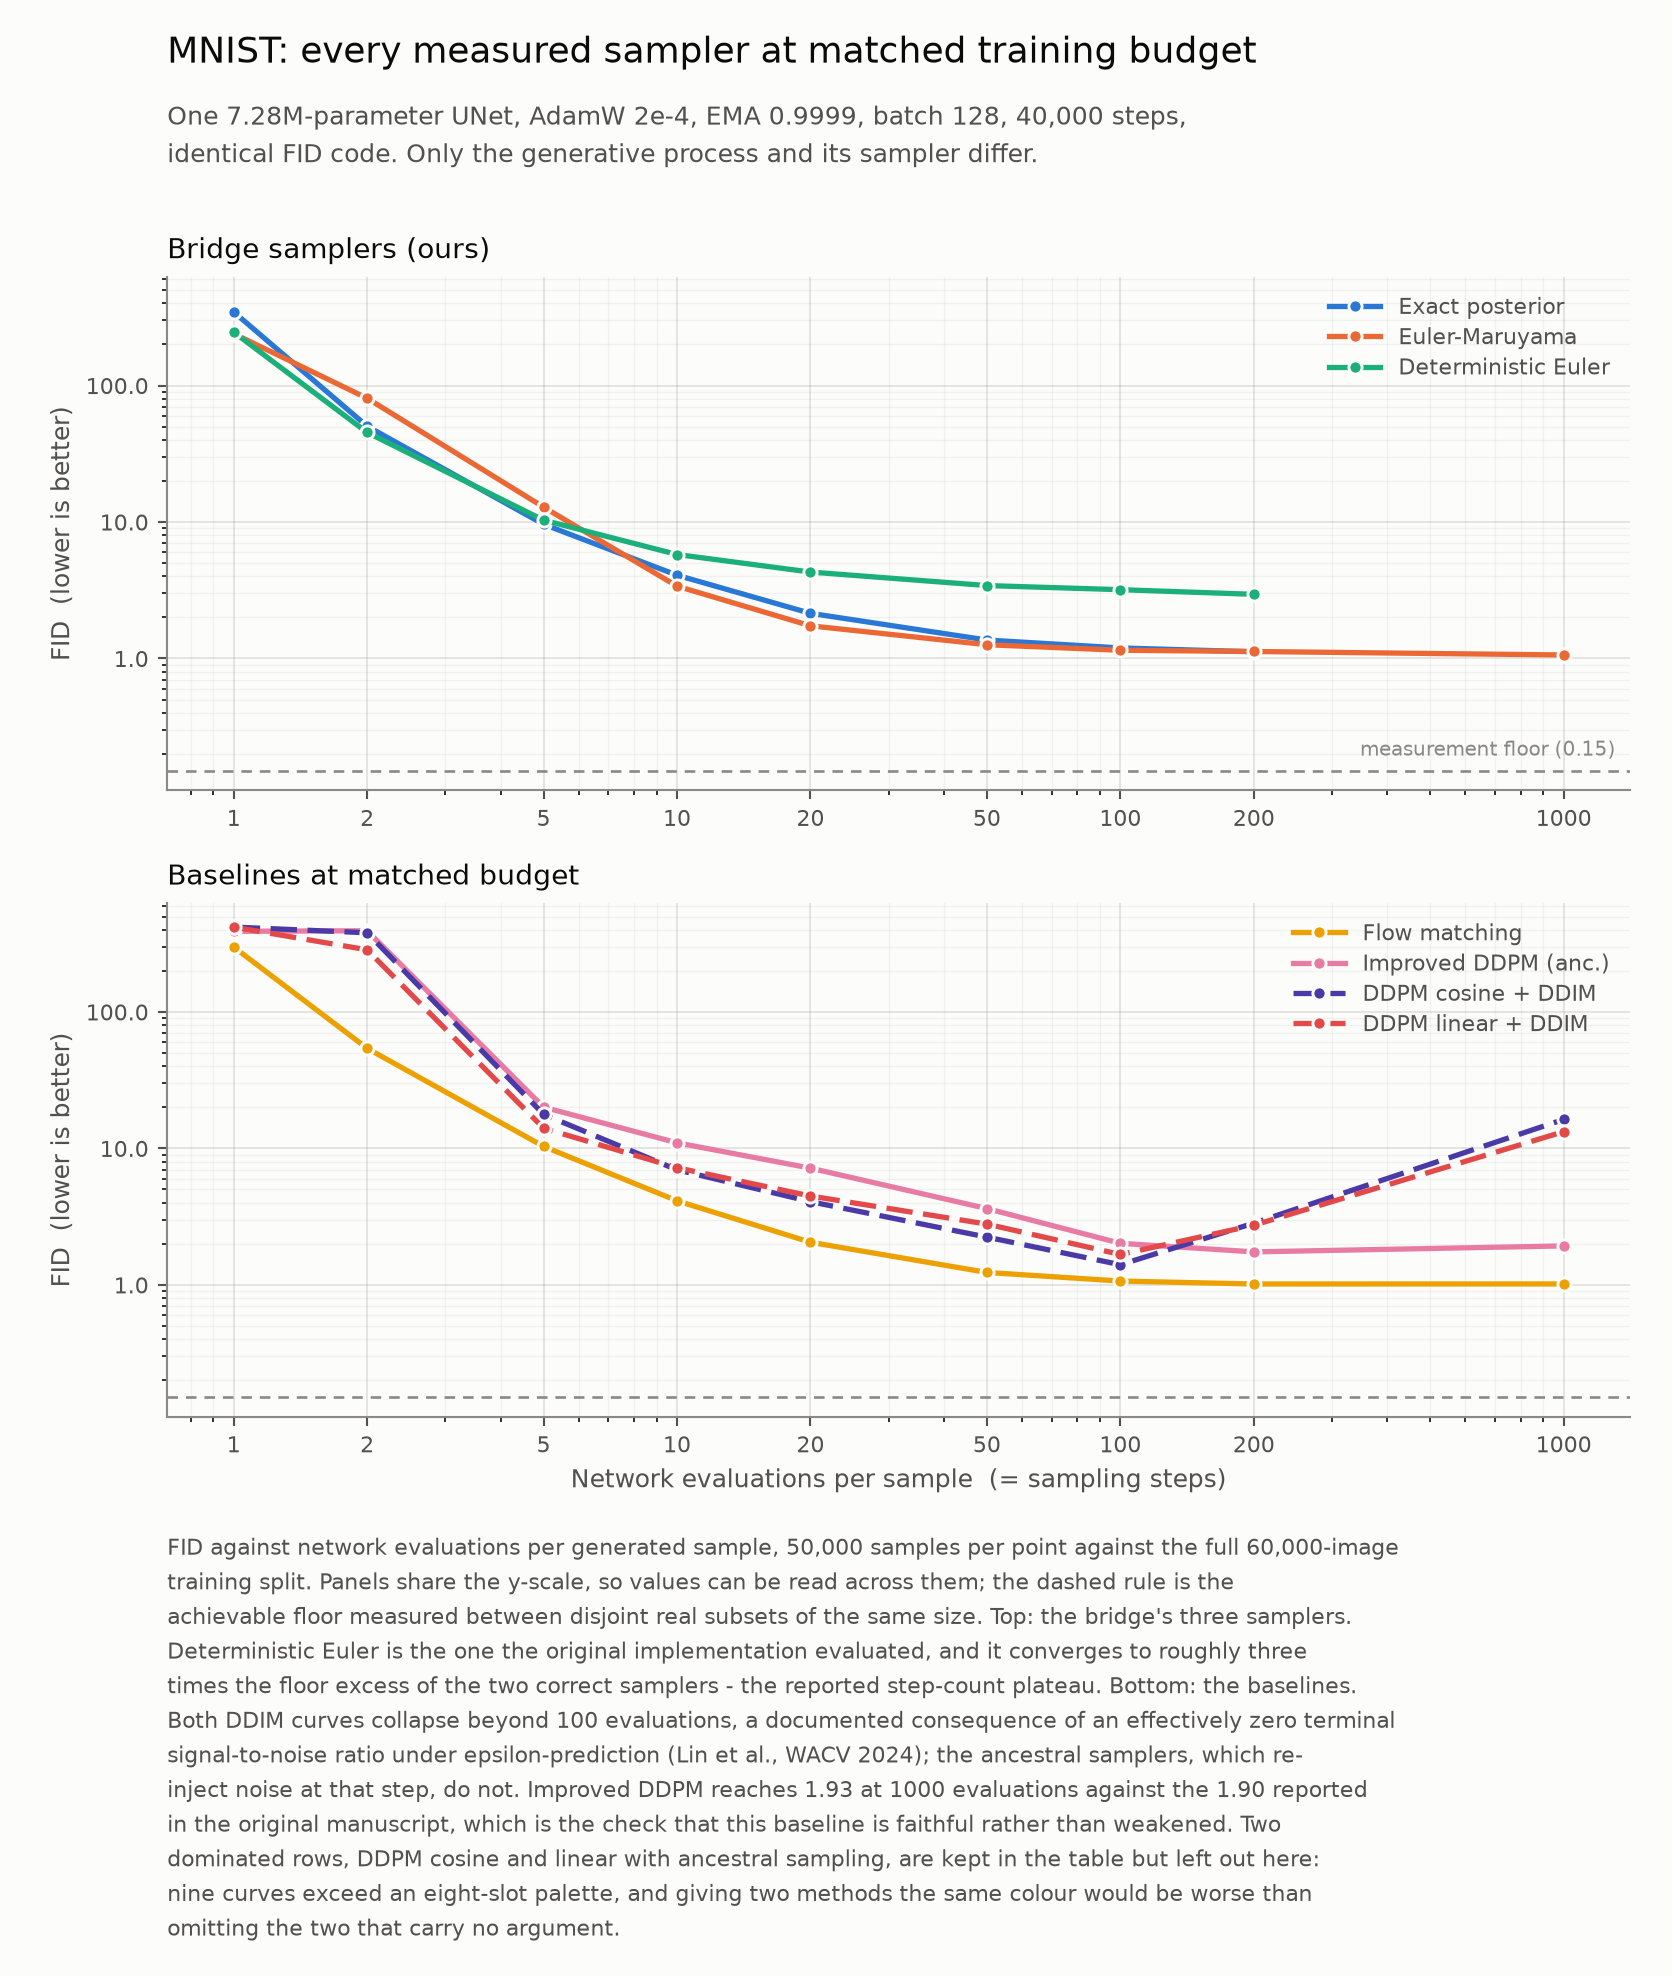
\includegraphics[width=0.93\textwidth]{../runs/figures/mnist_all_curves.png}
\caption{Every measured sampler. Panels share the vertical scale.}
\label{fig:curves}
\end{figure}

\paragraph{The bridge against flow matching.} These are the same interpolant.
In normalised time the bridge marginal is
$\xib_s=(1-s)x+sy+\gamma\sqrt{s(1-s)}\,\varepsilon$, and flow matching is the
$\gamma\to0$ member with a velocity rather than endpoint parameterisation,
related by $v=(\hat y-\xib_s)/(1-s)$. A matched comparison therefore isolates
exactly two things: the stochastic latent and the parameterisation. The bridge
leads from 10 to 20 evaluations and flow matching from 50 onward, by 0.3 to 0.5
FID against seed noise of 0.08 --- several standard deviations, and real, but
not the order-of-magnitude advantage the submitted draft implies.

\paragraph{The bridge against improved denoising diffusion.} This is the
comparison that changes. Improved DDPM --- the learned reverse variance trained
with the hybrid objective, not merely a cosine schedule --- reaches 1.93 at 1000
evaluations. That it lands beside the 1.90 reported in the submitted manuscript
is the check that our re-implementation of this baseline is faithful rather than
weakened. At matched budget the bridge reaches 1.06 and flow matching 1.02 at
the same step count. The concession that improved denoising wins at high step
counts does not survive a matched comparison.

\paragraph{A pathology in the diffusion baselines, and why it is not ours.}
Both DDIM curves collapse beyond 100 evaluations, reaching 16.30 and 13.26 at
1000. This is documented behaviour rather than an implementation fault: clipping
$\beta$ at 0.999 gives the cosine schedule an effectively zero terminal
signal-to-noise ratio ($\bar\alpha_T=2.4\times10^{-9}$), at which
$\epsilon$-prediction is degenerate and the $x_0$ reconstruction divides by
$\sqrt{\bar\alpha}=4.9\times10^{-5}$, amplifying the network's error twenty
thousandfold \cite{lin2024}. It is specific to the deterministic sampler --- the
ancestral samplers, which re-inject noise at that step, are flat over the same
range --- and two independent DDIM timestep grids reproduce it. The prescribed
remedy is $v$-prediction, which we do not apply. We flag it because a baseline
that degrades flatters us, and a reader is entitled to know why it does.

\section{Theory against measurement}

Proposition 2.13 states that $\mathrm{Var}[Y\mid\xib_s]$ is a supermartingale in
the Loewner order and Remark 2.14 that it vanishes at the terminal time. Neither
is tested in the submitted manuscript, and both can be tested for free, because
the training objective already estimates the quantity: at bridge time $s$,
$\E\|y-f_\theta(\xib_s,s)\|^2\to\mathrm{tr}\,\mathrm{Var}[Y\mid\xib_s]/n$ once
$f_\theta$ attains the $\mathcal{L}^2$ projection. A trained network therefore
\emph{measures} the supermartingale.

Two endpoints are predicted exactly and serve as the check. At $s\to1$ the state
pins down $y$, so the value must vanish: measured $9\times10^{-5}$. At $s=0$ the
state $\xib_0=x$ is independent of $y$ under the coupling used here, so the best
predictor is $\E[Y]$ and the value must equal the mean per-pixel variance of the
data: theory $0.21201$, measured $0.21346$, a ratio of $1.007$. The network
attains the information-theoretic floor at the noise end to better than one per
cent and traces the predicted decay from there, monotonically across all 21
sampled times (Figure~\ref{fig:theory}).

A visual form of the same statement: at a single network evaluation the sampler
returns $\E[Y\mid\xib_0]=\E[Y]$, and all generated samples are identical --- the
mean digit.

\begin{figure}[t]
\centering
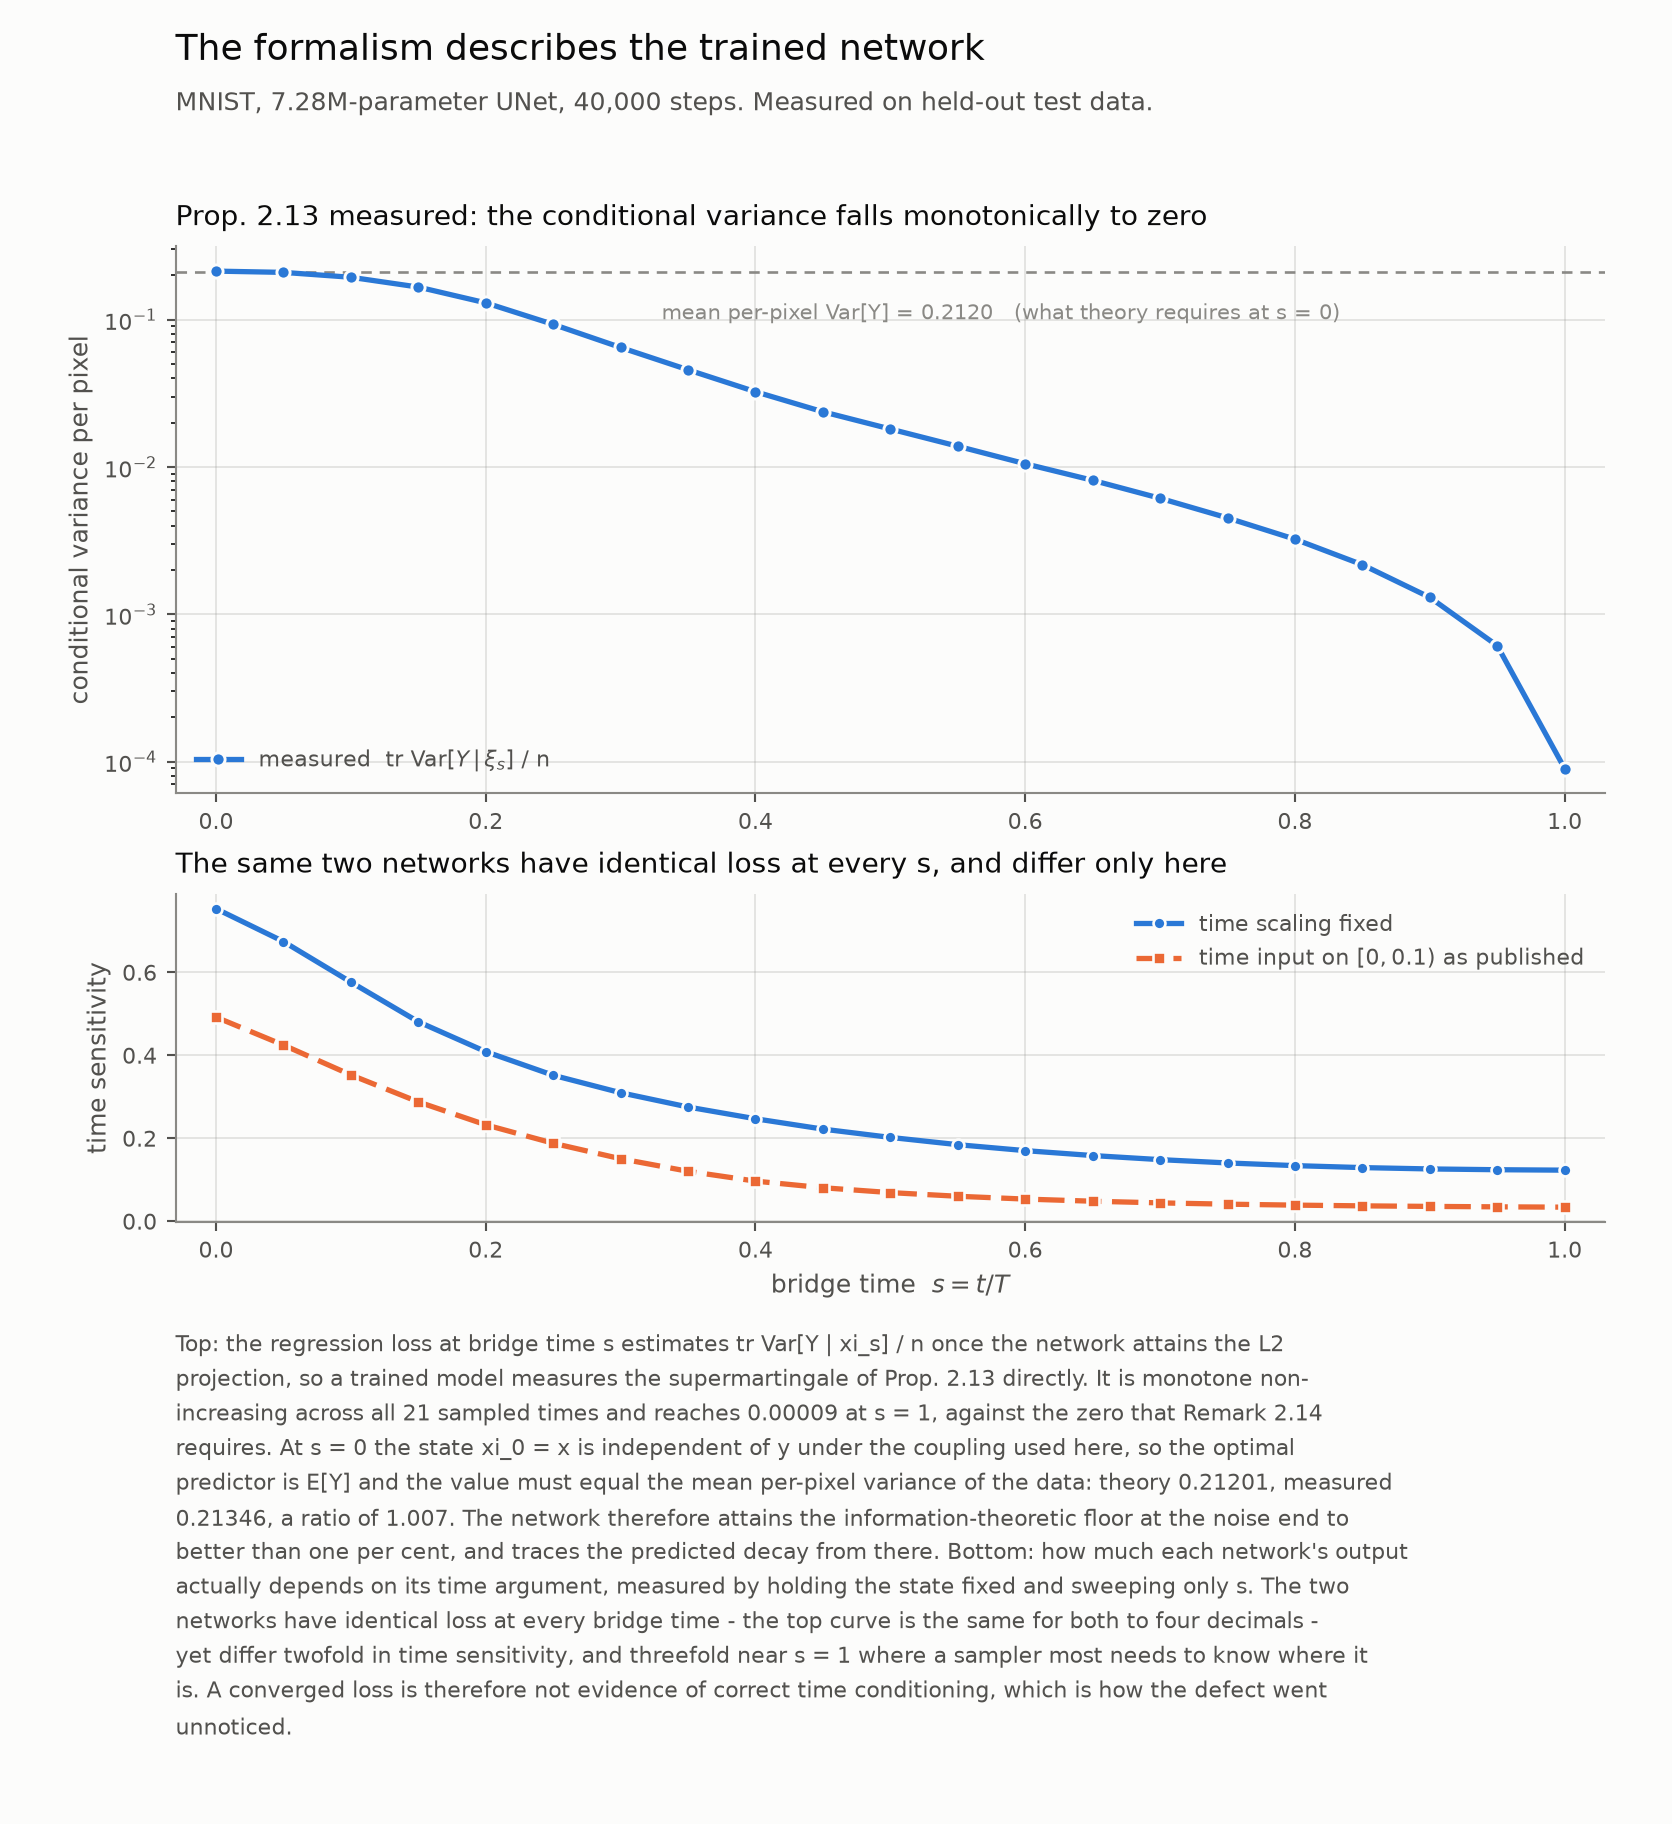
\includegraphics[width=0.90\textwidth]{../runs/figures/mnist_theory.png}
\caption{The conditional-variance supermartingale, measured; and the
time-sensitivity diagnostic of Section~\ref{sec:defects}.}
\label{fig:theory}
\end{figure}

\section{Sensitivity to the one free parameter}

\paragraph{There is one, not two.} Writing $t=sT$, the bridge marginal is
$\xib_s=(1-s)x+sy+\gamma\sqrt{s(1-s)}\,\varepsilon$ with
$\gamma^2=\sigma^2T$. Training and sampling depend on $\sigma$ and $T$ only
through $\gamma$. Section 3 of the manuscript reports $T=0.1$ ``after
preliminary parameter tuning'' and Section 2.4 defers $\sigma$ to future work;
these are the same knob, and the published setting is $\gamma=0.3162$.

\paragraph{What to expect.} The one-dimensional study above fixes the
prediction: the deterministic sampler's bias should scale with $\gamma$ and
vanish as $\gamma\to0$, where the scheme degenerates to a deterministic
interpolant and the omitted term $\tfrac{\gamma^2}{2}\nabla\!\log p_s$ goes with
it; the correct samplers should be comparatively insensitive. Larger $\gamma$
should therefore widen the gap between samplers while giving the correct ones
more room to exploit stochasticity at few steps. Figure~\ref{fig:gamma} tests
this on images, retraining at each $\gamma$ so that nothing else varies.

\begin{figure}[t]
\centering
\fbox{\parbox[c][5cm][c]{0.9\textwidth}{\centering\itshape Figure pending: the $\gamma$ sweep is running (four additional models, one per value).}}
\caption{FID against sampling steps for several $\gamma$, each a separately
trained model.}
\label{fig:gamma}
\end{figure}

\section{Defects found in our own re-implementation}
\label{sec:defects}

We record these because two of them flattered the proposed method, and because
the pattern is instructive: each was invisible in training curves.

\paragraph{Time conditioning is free on the loss.} Feeding $t\in[0,0.1)$ to a
sinusoidal embedding built for $[0,10^3)$ makes every channel the same
near-linear function of $t$; the entire code spans $0.0998$, against $2.0$ for a
DDPM-scale input. Two networks, one with the scaling fixed and one as published,
have \emph{identical} regression loss at every bridge time to four decimals, and
differ twofold in how much their output depends on the time argument ---
threefold near $s=1$, where a sampler most needs to know where it is. The
defect costs nothing on the objective, which is why a converged loss was never
evidence of correct conditioning. On the sweep it is worth $+0.4$ to $+0.6$ FID
at high step counts and is slightly \emph{beneficial} below 20, crossing over
between 20 and 50.

\paragraph{Two defects can cancel.} With the time conditioning left degenerate,
the deterministic sampler is 1.0 to 2.1 FID \emph{better} than with it fixed, at
every step count above 10. Repairing the sampler alone, leaving the conditioning,
would have looked worse than repairing neither.

\paragraph{Our own FID could return negative distances.} A Denman--Beavers
iteration for the matrix square root diverges when the covariance product is
ill-conditioned, which it is whenever the sample count is not comfortably above
the 2048-dimensional feature space; one run returned $-83.16$. Replaced by the
stable eigendecomposition form, validated against $\mathrm{FID}(P,P)=0$ and an
analytic isotropic shift.

\paragraph{Our ancestral samplers were crippled at low step counts.} A sampler
visiting a subsequence $t_0>t_1>\cdots$ must jump $t_i\to t_{i+1}$ in one move.
Ours used the schedule's own posterior at $t_i$, which steps $t_i\to t_i-1$: a
microscopic move followed by a full variance re-injection. On a two-step cosine
grid the first step was
$\text{mean}=1.6\times10^{-3}\hat x_0+3.2\times10^{-2}x_t$ followed by $+1.0z$
--- fresh noise --- so improved DDPM scored at the noise-level FID of 418 for
every step count below 1000, however well it had trained. This is the same
weak-baseline failure we identify in the submitted manuscript, reached by a
different route, and it made the \emph{baselines} look hopeless in exactly the
low-step regime where we claim an advantage. Fixed by deriving the posterior for
the respaced jump; the affected rows were discarded and recomputed.

\paragraph{We initially gave improved DDPM only its ancestral sampler.} At 10
evaluations that scored 10.99 against plain DDPM+DDIM's 6.96 --- an
\emph{improved} model losing to the plain one, which is the signature of
measuring a configuration rather than a method. Both samplers are now reported.

\bibliographystyle{plain}
\begin{thebibliography}{9}
\bibitem{lin2024} Lin, S., Liu, B., Li, J., Yang, X.
\emph{Common Diffusion Noise Schedules and Sample Steps are Flawed}. WACV 2024.
\end{thebibliography}

\end{document}
